\documentclass[11pt,a4paper]{article}
\usepackage[italian]{babel}
\usepackage[T1]{fontenc}
\usepackage[utf8]{inputenc}
\usepackage{graphicx}
\usepackage{imakeidx}
\usepackage{amsmath}
\usepackage{tabto}
\makeindex[intoc]
\usepackage[hyperfootnotes=false, colorlinks=true, linkcolor=black]{hyperref}


\begin{document}
\title{Concetti base UX design}
\author{Jacopo De Angelis}
\maketitle
\tableofcontents
\pagebreak

\begin{center}
	\begin{large}
		RIASSUNTO TESI 
		“SEGNI GRAFICI NELLA COMUNICAZIONE DEGLI ELETTRODOMESTICI: STUDIO E TASSONOMIA”
	\end{large}
\end{center}
\pagebreak

\section{Principi di design}
\subsection{I sette stadi dell'azione}
Un’azione è composta da due aspetti: la sua esecuzione e la valutazione dei suoi effetti e conseguenze.
Sette stadi principali di azione:
\begin{enumerate}
	\item \textbf{Scopo} (definizione dell’obiettivo)
	\item \textbf{Progettare} (definizione dell’azione da compiere)
	\item \textbf{Specificare} (definizione di una specifica sequenza di sotto-azioni)
	\item \textbf{Eseguire} (esecuzione dell’azione)
	\item \textbf{Percepire} (percezione dello stato del mondo)
	\item \textbf{Interpretare} (interpretazione dello stato del mondo)
	\item \textbf{Confrontare} (confronto tra il risultato ottenuto e lo scopo prefissato)
\end{enumerate}
Sei principi fondamentali del design ergonomico:
\begin{enumerate}
	\item \textbf{Visibilità}: permette all’utente di individuare facilmente qual è la 	funzione dell’oggetto, e quindi riconoscere se è adatto allo scopo prefissato. È il risultato dell’applicazione di tutti gli altri principi elencati.
	\item \textbf{Modello concettuale}: è il modello che l’utente ha dell’oggetto in questione; il modello può essere superficiale e riferirsi alla sola conoscenza di relazione tra input e output, ma può anche essere più approfondito, arrivando a conoscere anche tutti i passaggi intermedi a livello macchina. Più il modello concettuale è fedele al funzionamento reale, maggiore è la probabilità di successo nell’interazione tra utente e macchina.
	\item \textbf{Affordance} (invito all’uso): la relazione tra le azioni possibili di un agente in un determinato ambiente (JJ Gibson, 1979);
	\item \textbf{Significanti}: tutto ciò che aggiunge ulteriori indicazioni sull’esecuzione dell’azione, come direzione di movimento, senso di rotazione, ecc.
	\item \textbf{Feedback} (reazione): è l’insieme di risposte che il sistema comunica all’utente, in base alle azioni effettuate fino a quel momento.
	\item \textbf{Mapping}: è il rapporto fra i comandi, il loro azionamento ed i risultati che ne derivano nel mondo esterno; permette all’utente di creare un collegamento diretto fra i comandi di controllo e le parti dell’oggetto di cui modificano rispettivamente lo stato.
\end{enumerate}
\subsection{Il modello concettuale}
Il primo e forse più importante principio da tenere bene a mente è il modello concettuale, ovvero il modello di funzionamento dell’oggetto con cui l’utente si trova a interagire.
Un modello concettuale simile al modello di funzionamento reale fornisce all’utente la certezza sulle conseguenze delle proprie azioni, garantendo così un senso di controllo e di confidenza che migliora l’interazione. 
Al contrario, un modello concettuale distante dal modello di funzionamento reale può portare a effetti indesiderati da parte dell’utente, con conseguente senso di impotenza e frustrazione: emozioni che possono spingere ad abbandonare l’uso dell’oggetto in questione.
Una volta che l’utente ha ben chiaro il modello concettuale per stabilire il proprio piano d’azione, avviene la fase successiva: come può l’utente capire le possibilità di interazione con l’oggetto?
\subsection{Affordance}
L’affordance (invito all’uso) è stata definita da J.J. Gibson1 nel 1979 come la relazione tra le azioni possibili di un agente in un determinato ambiente; si può anche definire come la caratteristica di un oggetto che suggerisce all’utente le azioni appropriate per utilizzarlo. Un esempio semplice di affordance è dato dai bottoni: con la loro forma che si proietta al di fuori di una superficie piana uniforme, attirano l’attenzione e suggeriscono all’utilizzatore di premerli.
\subsection{Feedback}
Il feedback è uno strumento indispensabile per l’utente, in quando gli permette di comprendere le conseguenze delle proprie azioni, distinguendo un’azione corretta da una sbagliata in base al tipo di effetto ottenuto.
Un esempio di feedback è la luce che, nei forni a incasso, indica l’avvenuto raggiungimento della temperatura impostata dall’utente: l’accensione della spia dedicata è un ottimo modo per informare l’utente che ha raggiunto il primo obiettivo della sua operazione, ovvero riscaldare il forno.
I feedback sono importanti anche per capire quando è possibile procedere nelle operazioni con quel particolare oggetto.
\subsection{Mapping}
\begin{figure}
	\begin{center}
		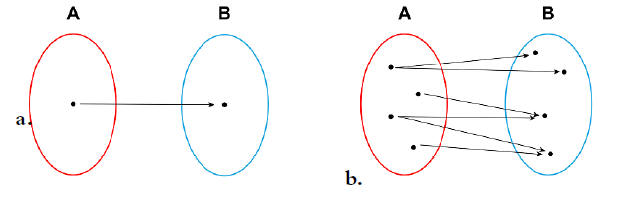
\includegraphics[scale=0.6]{img/001.png}
	\end{center}
	\caption{Mapping tra elementi di due insiemi}
\end{figure} 
"Mapping" è un termine tecnico che, nell’ambito matematico, indica la relazione fra gli elementi di due sistemi.
Un esempio semplice di mapping si può avere pensando al sistema di illuminazione domestico: il sistema A, costituito dagli interruttori elettrici, regola l’accensione e lo spegnimento del sistema B, costituito dai vari punti luce.
In questo caso possono venirci in aiuto i significanti, aggiungendo una targhetta sotto ogni interruttore che faccia riferimento al rispettivo punto luce controllato.
Per spiegare in modo più chiaro come il mapping può influenzare profondamente l’interazione uomo-oggetto, è possibile analizzare il piano cottura delle cucine. 
\begin{figure}
	\begin{center}
		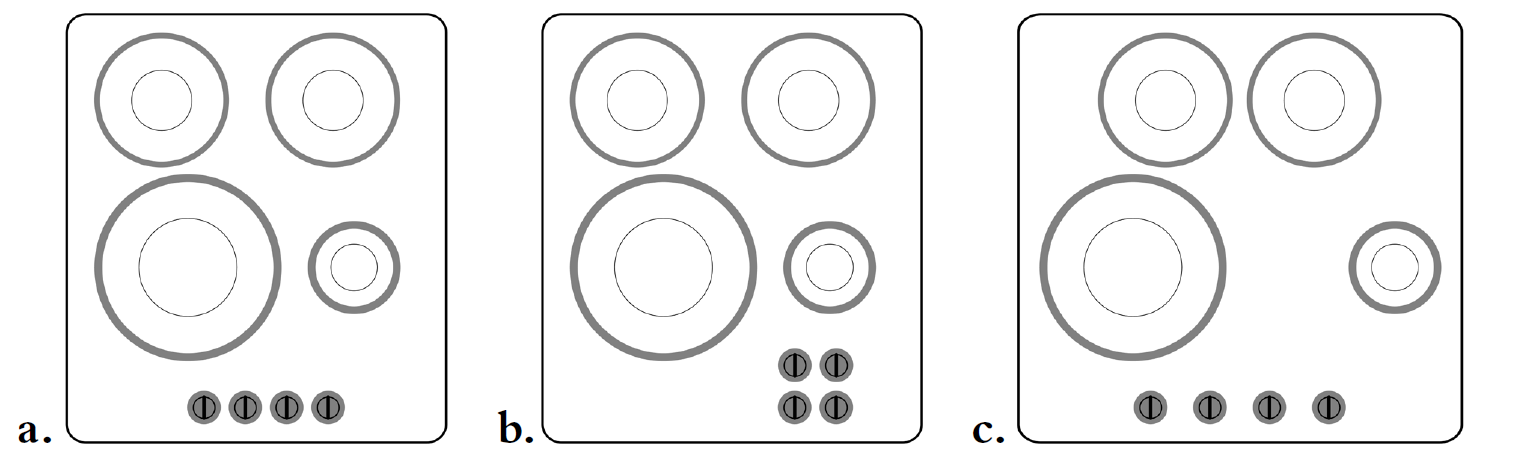
\includegraphics[scale=0.3]{img/002.png}
	\end{center}
	\caption{Schema di fornelli per cucinare}
\end{figure}
Il più comune piano cottura è composto da 4 fornelli disposti ai vertici di un quadrato, ciascuno controllato da una delle manopole circolari, generalmente disposte in sequenza.
\pagebreak
\section{Interfacce e interazione}
L’interfaccia qui presa in esame, dunque, fa riferimento a tutta quella serie di componenti che permettono l’interazione uomo-macchina in due sensi:
\begin{itemize}
	\item uomo --> macchina: l’utente ha la possibilità di gestire i comandi e le funzioni della macchina per raggiungere il proprio obiettivo (avviare un programma della lavatrice per lavare i panni, scaldare il forno per cucinare una pietanza, ecc.);
	\item Macchina --> uomo: la macchina comunica i propri cambiamento di stato all’utente (nel forno si accende una luce rossa una volta raggiunta la temperatura desiderata, viene emesso un suono ripetuto una volta scaduto un timer impostato, ecc.).
\end{itemize}
\subsection{Interazione uomo macchina}
\begin{figure}
	\begin{center}
		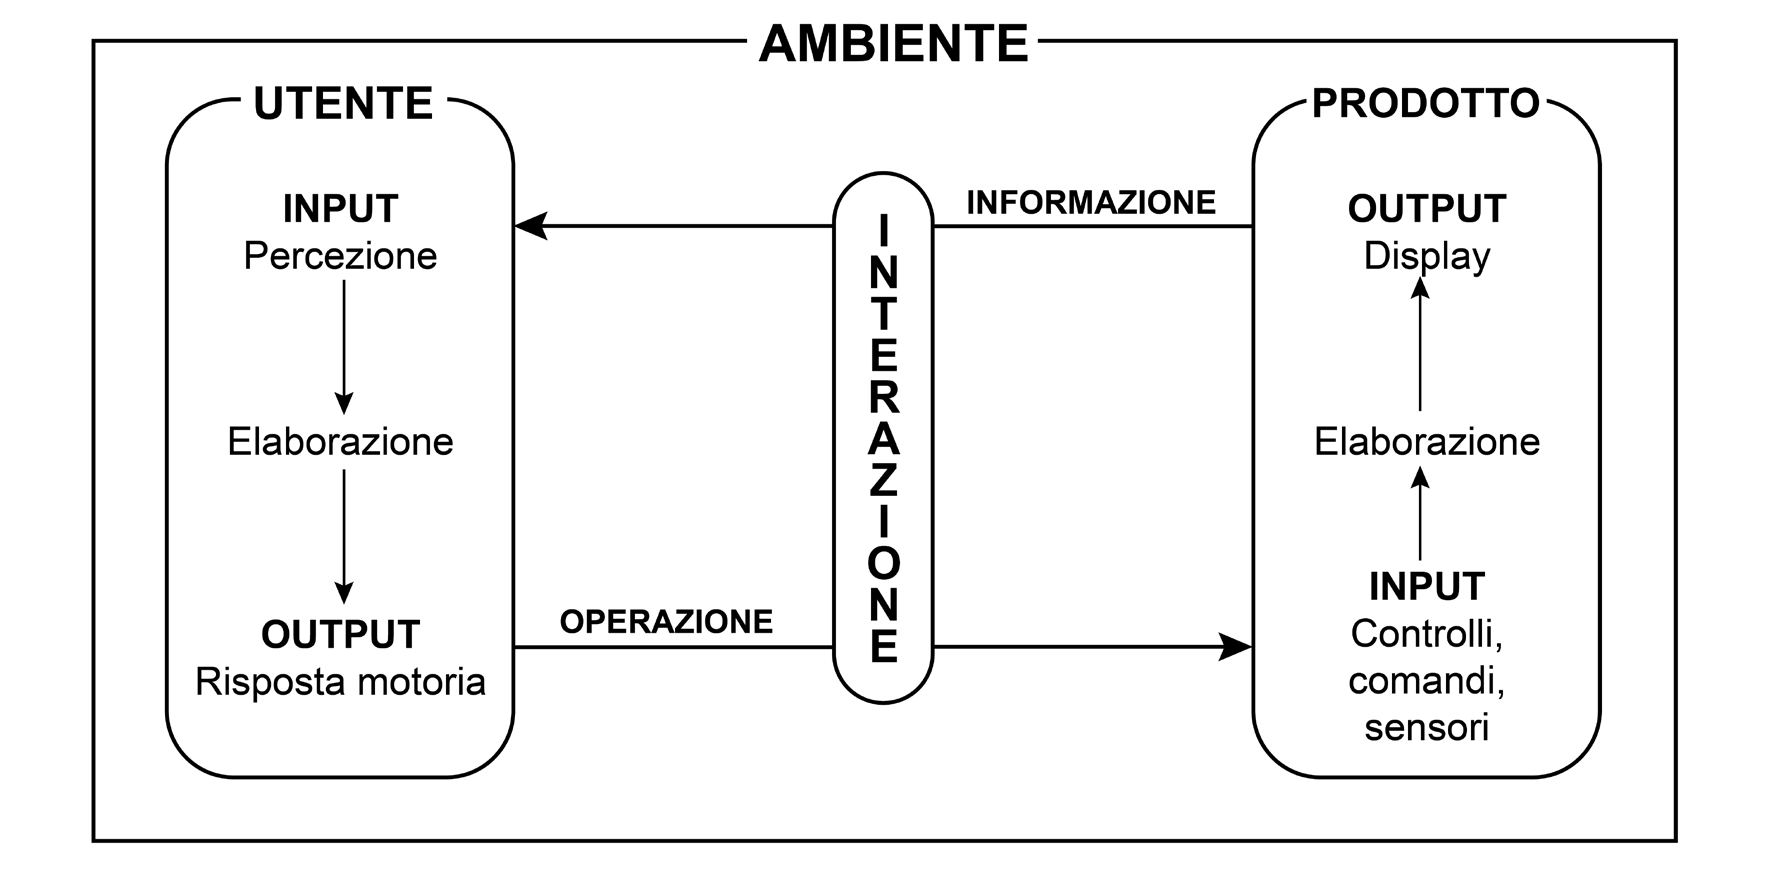
\includegraphics[scale=0.3]{img/003.png}
	\end{center}
	\caption{L'interazione utente-prodotto}
\end{figure}
Chiaramente che l’interazione non è a “senso unico”: è infatti rappresentato un ciclo di operazioni che vanno dall’utente al prodotto e viceversa. Analizziamo più nel dettaglio questo ciclo, utile per comprendere in che modo la comunicazione tra utenti e oggetti è fondamentale per un’esperienza corretta e soddisfacente.
\begin{itemize}
	\item Prodotto --> informazione (output): Le informazioni, una volta comunicate dall’oggetto tramite gli appositi canali sensoriali (visivo, sonori, tattili), vengono percepite dall’utente attraverso gli organi di senso.
	\item Informazione --> utente (percezione): L’utente, una volta recepite le informazioni, deve rielaborarle e convertire quei “segnali” in dati utili e dotati di senso: l’accensione di determinate spie, ad esempio, veicola un informazione precisa sullo stato del prodotto che l’utente deve riconoscere.
	\item Utente = elaborazione: L’elaborazione delle informazioni porta l’utente a programmare le azioni da svolgere sull’oggetto per poter portare a termine il proprio scopo. Seguirà quindi una risposta motoria che può coinvolgere diversi sensi a seconda del tipo di interazione prevista dal prodotto: comandi vocali, comandi di posizione spaziale, pulsanti, manopole, schermi sensibili al tocco ecc.
	\item Utente --> operazione (output): Questa risposta motoria da parte dell’utente si concretizza nell’interazione diretta con il prodotto: girare una manopola, premere un pulsante, impartire uno specifico comando vocale.
	\item Informazione (input) --> prodotto: Questi comandi fungeranno da input per la macchina, che a sua volta li elaborerà per poi portare a termine le richieste dell’utente.
	\item Prodotto = elaborazione: Una volta elaborati gli input dell’utente e avviate le proprie operazioni, la macchina dovrà comunicare all’utente il proprio stato, ricominciando il ciclo.
\end{itemize}
In ciascuna delle fasi appena descritte possono verificarsi problemi che inficiano l’esperienza e l’interazione con l’oggetto.
\begin{itemize}
	\item Prodotto --> informazione (output)
		\tab L'informazione può essere comunicata in modo inefficace, insufficiente o non essere affatto comunicata. Questo è il caso di elementi difettosi, come led bruciati che non si accendono o altoparlanti guasti che non emettono allarmi acustici. Sotto l’aspetto dell’interfaccia questi problemi possono essere arginati sfruttando più canali di comunicazioni: ad esempio un led e un segnale acustico possono comunicare insieme lo stesso messaggio e, qualora uno dei due canali fosse mancante, l’altro potrebbe sopperire. Non bisogna però incorrere nell’eccesso, sovraccaricando così gli stimoli dell’utente con troppe informazioni simili in contemporanea.
	\item Informazione --> utente (percezione)
		\tab L’informazione può essere percepita in modo distorto dall’utente, o può non essere percepita affatto. Ad esempio un utente caratterizzato da daltonia potrebbe non distinguere due luci una di colore verde e l’altra di rosso.In altri casi le informazioni rilevanti potrebbero essere comunicate insieme ad altre meno importanti, rischiando quindi di essere trascurate parzialmente o completamente.
Per ovviare a questi problemi è consigliabile selezionare accuratamente le informazioni più importanti da comunicare all’utente, e cercare di renderle per chiare e distinguibili; anche in questo caso si possono sfruttare diversi canali di comunicazione, stando attenti a non confondere l’utente e a non sovraccaricarlo.
	\item Utente = elaborazione
		\tab In questa fase l’utente raccoglie e rielabora i dati raccolti attraverso gli organi di senso, e per farlo sfrutta le proprie capacità cognitive per organizzare un pensiero da tramutare in azione, sempre sulla base del proprio scopo. Il progettista in questo caso non ha il controllo dell’operazione, in quanto dipende dal soggetto in questione e possono influire numerose variabili. Si possono però tenere a mente alcune di queste variabili così da ridurre il flusso iniziale di informazioni, cercando di comunicare con chiarezza, evitando possibili fraintendimenti e selezionando le funzioni più rilevanti per l’utente.
	\item Utente --> operazione (output)
		\tab Una volta elaborato il tipo di azione da svolgere, l’utente potrebbe avere difficoltà a comprendere come elaborare quel’idea in un’azione concreta sull’oggetto. Per questo motivo è essenziale rendere ben evidenti e accessibili i comandi di controllo dell’interfaccia, come cursori, manopole e pulsanti; non solo devo essere visibili, ma è indispensabile che siano facilmente accessibili. Infine bisogna sempre rendere chiaro l’effetto che i comandi di controllo hanno sulla macchina: per questo motivo è consigliabile raggruppare comandi, spie e indicazioni inerenti la stessa funzione, così da aiutare nella scelta e scongiurando fraintendimenti o confusione.
	\item Prodotto = elaborazione
		\tab Il prodotto avrà il compito di elaborare gli input dell’utente e portare a termine le operazioni richieste. Nuovamente possono sorgere problemi di natura sistemica: pezzi malfunzionanti, parti disconnesse, e così via.
\end{itemize}
\begin{figure}	
	\begin{center}
		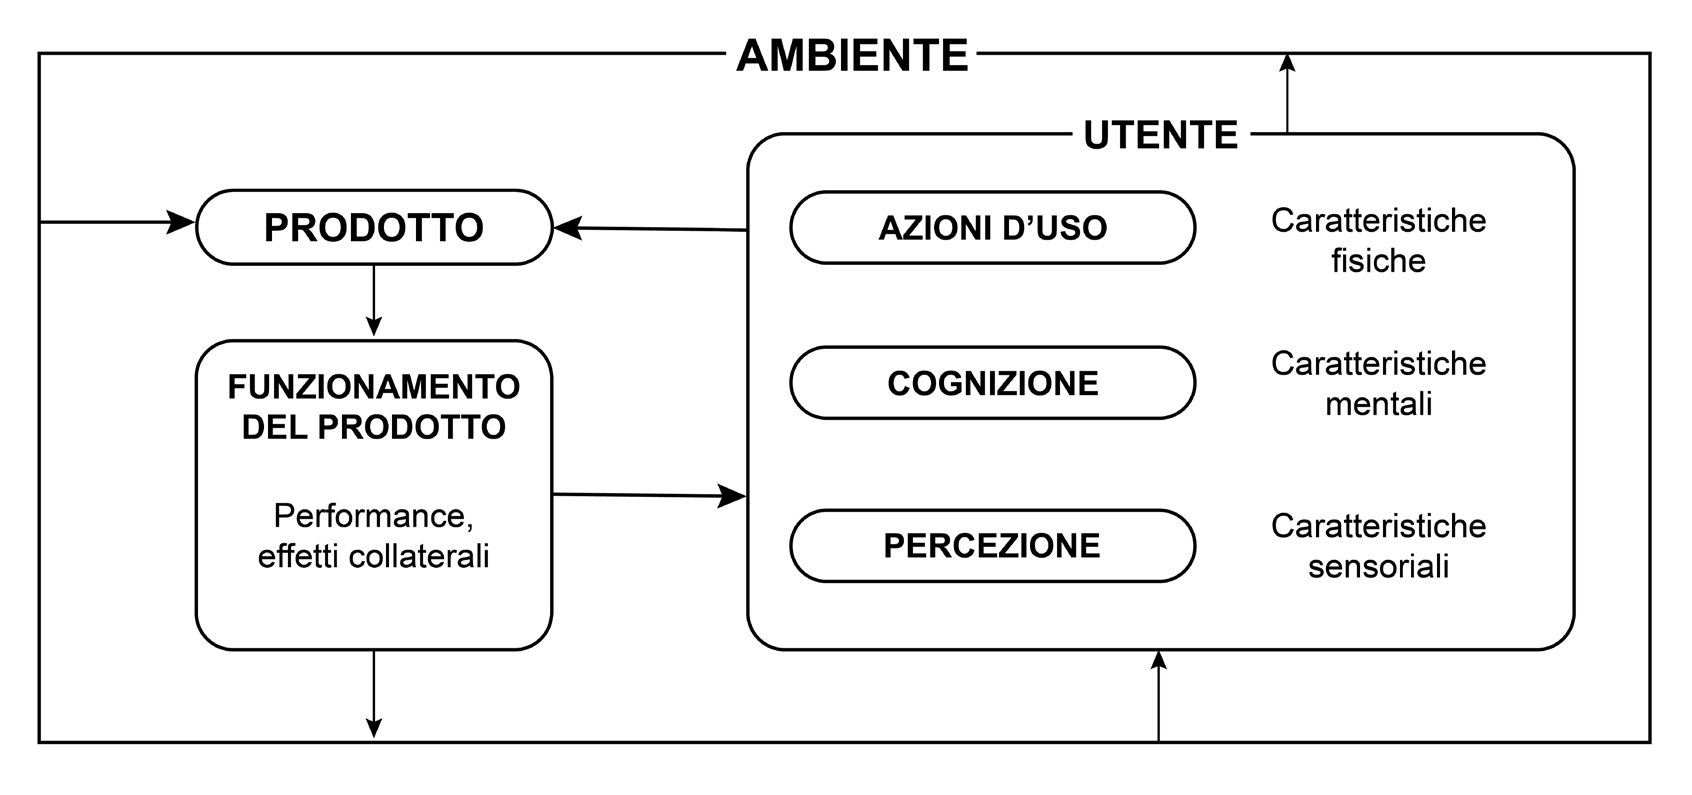
\includegraphics[scale=0.4]{img/004.png}
	\end{center}
	\caption{L'interazione utente-prodotto}
\end{figure}
Dal momento che, come abbiamo visto, la percezione è alla base della comunicazione, bisogna ricordare che il cervello è selettivo per quanto riguarda tutte le informazioni che riceve contemporaneamente, filtrandole e selezionando quelle più rilevanti attraverso tre processi percettivi:
\begin{itemize}
	\item \textbf{Attenzione selettiva}: malgrado ciascuno di noi sia esposto a numerosi e variegati stimoli (stimoli acustici, visivi, tattili, di diversa intensità e natura), la nostra attenzione si focalizza su stimoli legati a bisogni del momento, a stimoli particolarmente intensi o diversi dalla norma o ancora a stimoli particolarmente attesi.
	\item \textbf{Distorsione selettiva}: gli stimoli filtrati vengono rielaborati differentemente a seconda dell'individuo, sulla base delle singole capacità cognitive, esperienze, influenze culturali ecc.
	\item \textbf{Ritenzione selettiva}: solo una piccola parte di quello che viene percepito viene memorizzato, in base allo stato emotivo e cognitivo che ha accompagnato la rielaborazione.
\end{itemize}
Quattro fattori principali in ordine di influenza:
\begin{itemize}
	\item \textbf{Fattori culturali}: sono "quelli che esercitano sull'individuo un'influenza più ampia e profonda; la cultura è l'insieme di strumenti tanto mentali quanto fisici, progettati dall'uomo, che rappresentano i modelli di vita di un gruppo, di una classe, di una società" (Lina Bonapace, "La piacevolezza", contenuto in "Progettazione ergonomica", Francesca Tosi, Il Sole 24 Ore, Milano, 2001). La subcultura è "costituita da un gruppo che, all'interno di una data società, condivide le principale caratteristiche di questa, ma presenta valori, abitudini e tradizioni distinguibili come propri."
	\item \textbf{Fattori sociali}: derivano dai gruppi di riferimento, ovvero dei gruppi che possono esercitare un'influenza sui comportamenti degli individui. L'influenza può essere esercitata in modo diretto, per esempio all'interno della famiglia, attraverso l'adozione di regole e abitudini particolari, oppure in modo indiretto tramite l'aspirazione a determinati modelli di vita.
	\item \textbf{Fattori personali}: l'età, le caratteristiche fisiche, le condizioni economiche. Ciascuno di questi fattori muta sensibilmente il rapporto dell'individuo con il mondo esterno, rendendolo più o meno sensibile a determinati stimoli, più o meno predisposto a determinate attività: ad esempio, operazioni fisicamente impegnative risulteranno più facili per individui allenati.
	\item \textbf{Fattori psicologici}: motivazione, percezione, apprendimento, credenze.
\end{itemize}
\subsection{Complessità, controllo automazione}
Le funzioni più importanti o utilizzate più frequentemente in un prodotto complesso possono essere accessibili istantaneamente tramite la pressione di un pulsante comodo e ben visibile (hard key). Le funzioni utilizzate meno frequentemente potrebbero essere accessibili in un modo meno diretto:
\begin{itemize}
	\item Pulsanti più piccoli, magari nascosti sotto uno sportello apribile
	\item Tenendo premuto uno o più pulsanti
	\item Tramite una soft key, ovvero un pulsante la cui funzione cambia a seconda di una grafica mostrata in un display vicino
	\item Attraverso la selezione in un menù 
\end{itemize}
Infine non mancano considerazioni sul tipo di controllo, diverso a seconda del tipo di funzione a cui fa riferimento. In particolare:
\begin{itemize}
	\item Funzioni che sono analogiche e che possono variare su scala "continua" godono una implementazione tramite controlli analogici o continui (manopole e cursori)
	\item Funzioni che richiedono una singola azione "discreta" vengono implementate al meglio tramite pulsanti
	\item Funzioni che richiedono una selezione tra molteplici impostazioni "discrete" vengono implementate al meglio con cursori, manopole o rotelle che producono uno scatto in ogni posizione, oppure con un pulsante usato per scorrere ("alternare") l'attivazione di opzioni indicate da un display nelle vicinanze.
\end{itemize}

\section{Psicologia della Gestalt}
\subsection{Principio dell'emergentismo}
\begin{figure}
	\begin{center}
		
\includegraphics[scale=0.3]{img/005.png}
	\end{center}
	\caption{Esempio di emergentismo: macchie di colore nello spazio vengono
percepite come la rappresentazione di un dalmata}
\end{figure}
L'emergentismo (o comportamento emergente) è una teoria secondo cui un sistema complesso mostra comportamenti e proprietà ben definite, ma che risultano difficilmente prevedibili studiando i singoli elementi che lo compongono.
Nella Gestalt l'emergentismo è utilizzato per spiegare il modo in cui il nostro cervello elabora gruppi di elementi, spesso senza attribuirne valore singolarmente, ma riconoscendo il sistema di cui fanno parte, ovvero percependo l'intero insieme prima delle singole parti che lo compongono.
\subsection{Principio della reificazione}
\begin{figure}
	\begin{center}
		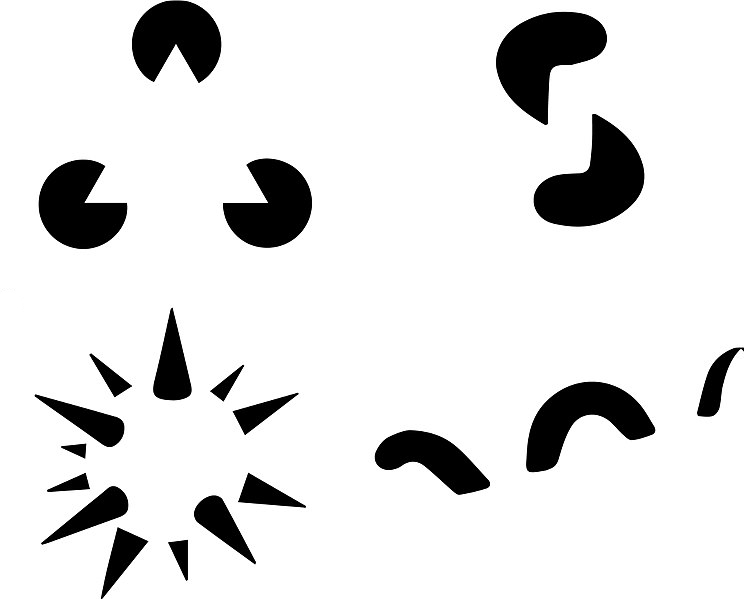
\includegraphics[scale=0.3]{img/006.png}
	\end{center}
	\caption{esempi di reificazione: a. il triangolo di Kanizsa, b. una S tagliata, c. una mazza chiodata, d. un mostro marino.}
\end{figure}
Nella disciplina della logica, la reificazione è una fallacia (o ambiguità) che si verifica quando un'astrazione, ovvero un costrutto ipotetico, viene considerato come un evento reale e concreto, o addirittura un'entità fisica.
Nella Gestalt la reificazione permette di spiegare come la percezione di determinati sistemi figurativi ci porti a vedere strutture anche dove non sono realmente presenti.
\subsection{Principio della multistabilità}
\begin{figure}
	\begin{center}
		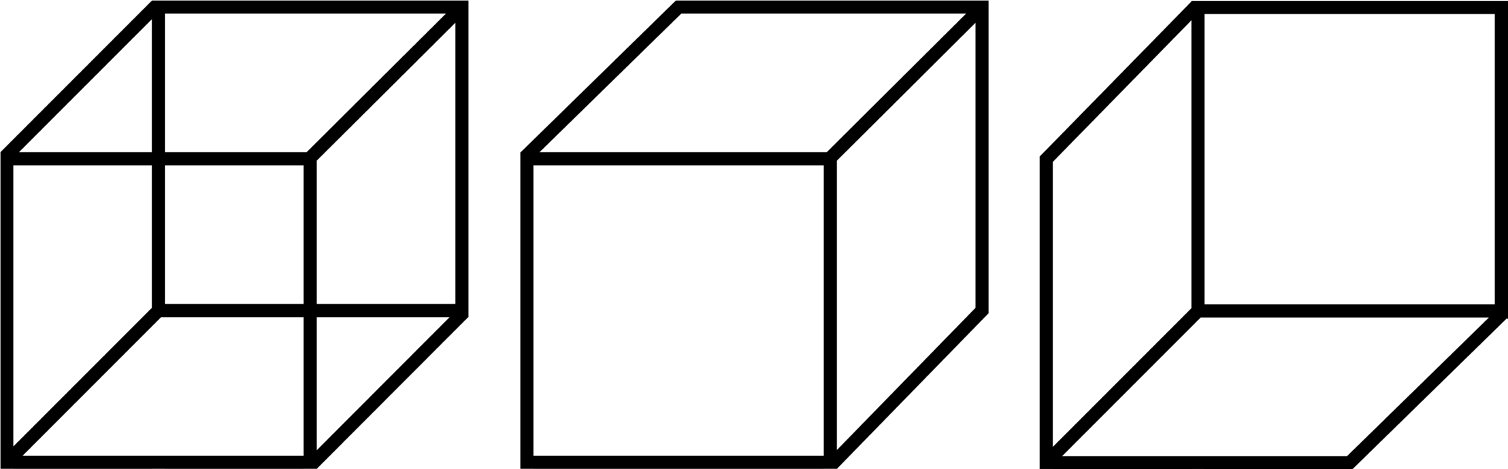
\includegraphics[scale=0.3]{img/007.png}
	\end{center}		
	\caption{Illusione ottica "cubo di Necker"}
\end{figure}
La multistabilità è un fenomeno per cui una figura viene percepita con significati differenti in momenti differenti, anche a breve distanza temporale. La multistabilità è alla base di numerose illusioni ottiche e ne esistono diversi esempi.
\subsection{Principio dell'invarianza}
\begin{figure}
	\begin{center}
		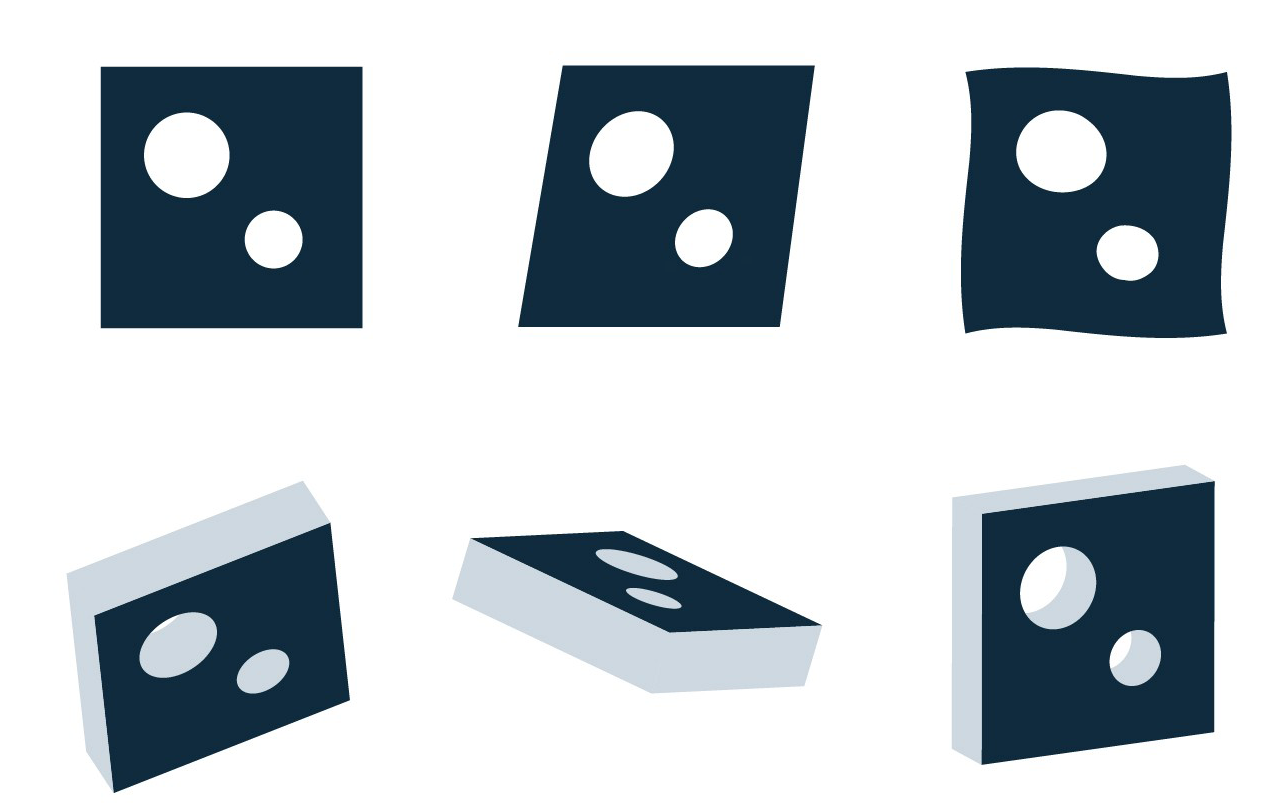
\includegraphics[scale=0.3]{img/008.png}
	\end{center}
	\caption{Esempio di invarianza}
\end{figure}
L'invarianza è una proprietà della percezione che permette di riconoscere oggetti indipendentemente dalla loro traslazione, rotazione e scala. Questo significa che è possibile riconoscere un oggetto anche in seguito a deformazioni che ne hanno cambiato l'apparenza rispetto alla prima volta in cui è stato incontrato.
\pagebreak
\subsection{Le otto leggi}
I quattro principi esposti precedentemente non si manifestano quasi mai singolarmente, ma è molto più comune incontrarli in diverse combinazioni, generando così particolari effetti. A partire da questi principi vengono declinate otto leggi differenti:
\begin{enumerate}
	\item \textbf{Legge della buona forma }(o della \textbf{pregnanza}, dal tedesco \textbf{pragnanz}): gli elementi visivi in un sistema vengono percepiti come forme semplici ed elementari. Quando sono presenti linee tra loro non continue, l'occhio tende a percepire gruppi di linee come figure semplici come poligoni convessi (triangolo, quadrato, cerchio, ecc.)
	\item \textbf{Legge di prossimità}: gli elementi visivi vengono percepiti in gruppi, in base alla loro distanza reciproca. Questo vuol dire che elementi distanti tra loro verranno percepiti come separati, senza alcune legame diretto di contenuto, mentre elementi tra loro vicini verranno percepiti come appartenenti a un gruppo omogeneo caratterizzato da proprietà comuni.
	\item \textbf{Legge di somiglianza}: gli elementi visivi all'interno di un sistema vengono percepiti com appartenenti a diversi gruppi in base alla condivisione di alcune proprietà. Elementi che hanno colore, forma o dimensioni simili verranno percepiti come un gruppo, e quindi considerati simili in termini di significato.
	\item \textbf{Legge di buona continuità}: gli elementi lineari di un sistema vengono percepiti secondo il percorso più continuo e lineare possibile, anche se caratterizzato da molteplici interruzioni. Anche quando due o più elementi lineari si intersecano, l'osservatore tende a vedere sempre percorsi continui, mentre è più difficile che percepisca oggetti con un percorso caratterizzato da cambi repentini di direzione.
	\item \textbf{ Legge di destino comune}: i singoli elementi di un sistema vengono percepiti come un gruppo disposto sul percorso più semplice e lineare possibile. Gli elementi vengono quindi raggruppati secondo l'appartenenza a un'immaginaria linea continua che li collega, e questa linea segue le regole della legge di buona continuità.
	\item \textbf{ Legge figura-sfondo}: all'interno di un sistema di elementi, è necessario per l'osservatore distinguere distintamente gli elementi che rappresentano la figura, in primo piano, dall'ambiente intorno che costituisce lo sfondo.
	\item \textbf{Legge di simmetria}: gli elementi di un sistema che sono percepiti come simmetrici vengono considerati come un tutt'uno, a prescindere dalla distanza. Questo fenomeno (così come la legge di continuità e quella di destino comune) è all'origine della ricerca di un ordine e di una coerenza nel sistema osservato.
	\item \textbf{Legge di chiusura}: gli elementi incompleti o interrotti vengono percepiti come un intero, anche se presenta frammentazioni. Questo fenomeno è simile alla pragnanz, in quanto l'osservatore tende a ricondurre gli stimoli visivi a figure semplici e facilmente riconoscibili.
\end{enumerate}
\subsection{Semiotica e interpretazione}
La semiotica è la disciplina che studia i segni e, più in particolare, studia proprio la semiosi, ovvero il processo tramite cui si attribuisce un senso o un significato a un segno. \\
\textbf{Segno}: \textit{qualcosa che sta per qualcuno al posto di qualcos'altro, sotto certi aspetti o capacità.} \\
Il Rapresentamen è qualcosa che sta al posto di qualcos'altro, ovvero per il suo Oggetto. Il Rapresentamen sta per l'Oggetto non sotto ogni aspetto possibile, ma solo a partire da una determinata scelta di pertinenza. \\
Per spiegare la pertinenza si può fare un esempio, prendendo un insieme qualunque di tre oggetti quotidiani: un bicchiere di carta, un posacenere di cristallo e un martello di acciaio. Questo insieme può essere suddiviso in diversi sottoinsiemi, a seconda del principio di classificazione scelto:
\begin{itemize}
	\item secondo il criterio "oggetti utili per contenere liquidi" possiamo costruire il sottoinsieme costituito dagli elementi posacenere e bicchiere
	\item secondo il criterio "oggetti che possono essere usati come arma di difesa" possiamo costruire il sottoinsieme che contiene gli elementi martello e posacenere.
\end{itemize}
Ne deriva che "la decisione di assumere un dato oggetto sotto un certa regola interpretativa (o abito interpretativo) invece che un altro dipende dall'universo di discorso nel quale ci si muove in quel determinato momento"1. La regola interpretativa, ovvero la pertinenza, da applicare dipende dal contesto. \\
Un'ulteriore distinzione è tra oggetto dinamico e oggetto immediato:
\begin{itemize}
	\item \textbf{Oggetto dinamico}: realmente efficiente ma non immediatamente presente
	\item \textbf{Oggetto immediato}: così come il segno lo rappresenta
\end{itemize}
In base a questa distinzione tra Oggetto Dinamico e Oggetto Immediato, possiamo definire il segno come la combinazione di un Rapresentamen (in quanto Espressione) e di un Oggetto Immediato (in quanto Contenuto del segno).
\begin{figure}
	\begin{center}
		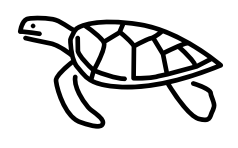
\includegraphics[scale=0.6]{img/009.png}
	\end{center}
	\caption{Disegno di una tartaruga}
\end{figure}
Quindi, per riassumere, basandosi sull'immagine appena vista:
\begin{itemize}
	\item il Rapresentamen corrisponde alla pura espressione grafica (ovvero la combinazione di punti, linee ed aree così come sono percepite dall'occhio umano);
	\item l'Oggetto Immediato equivale al concetto di "tartaruga" (ad esempio se contrapposto al concetto di "lepre" se si vuole esprimere un senso di lentezza/velocità);
	\item l'Oggetto Dinamico coincide con tutte le tartarughe "in carne e ossa" a cui il segno si riferisce, ovvero a tutte le tartarughe esistenti.
\end{itemize}
Vi sono ulteriori strumenti per l'interpretazione, una delle teorie è che l'immagine artistica sia composta da due tipi di linguaggi:
\begin{itemize}
	\item \textbf{Linguaggio figurativo}:  permette di riconoscere nell'immagine oggetti (e dunque significati) appartenenti direttamente al mondo esterno;
	\item \textbf{Linguaggio plastico}: permette di riconoscere dei significati nell'immagine che trascendono la mera rappresentazione figurativa della realtà
\end{itemize}
L'analisi plastica, che indaga il significato del linguaggio plastico, inizia con lo studio dell'organizzazione degli elementi dell'immagine sulla base di tre diverse categorie:
\begin{itemize}
	\item \textbf{categorie cromatiche}: riconoscendo i colori utilizzati e le loro caratteristiche (colori caldi/freddi, colori chiari/scuri, colori lucidi/opachi, luce/ombra, monocromatico/policromatico, ecc.)
		\begin{figure}
			\begin{center}
				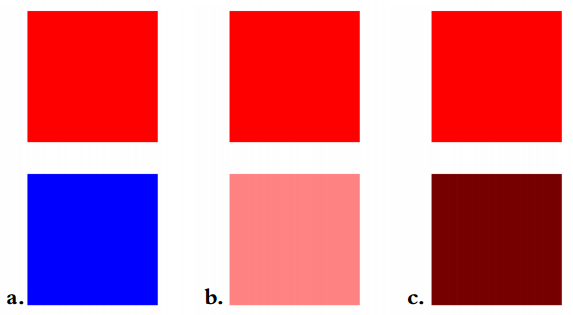
\includegraphics[scale=0.6]{img/010.png}
			\end{center}
			\caption{Esempi di categorie cromatiche: a. tonalità (rosso/blu), b. saturazione (saturo/desaturato), c. luminosità (chiaro/scuro).}
		\end{figure}
	\item \textbf{categorie eidetiche}: riconoscendo le linee nell'immagine e i loro rispettivi attributi (corto/lungo, continuo/segmentato, orizzontale/verticale, convergente/parallelo, curvilineo/rettilineo, ecc.)
		\begin{figure}
			\begin{center}
				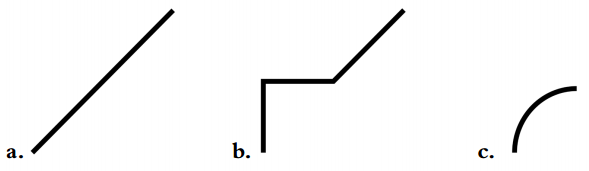
\includegraphics[scale=0.6]{img/011.png}
			\end{center}
			\caption{Esempi di categorie eidetiche: a. lungo+rettilineo+non segmentato, b. lungo+segmentato, c. corto+curvilineo}
		\end{figure}
	\item \textbf{categorie topologiche}: riconoscendo la relazione spaziale tra i vari elementi dell'immagine (destra/sinistra, alto/basso, circoscritto/circoscrivente, davanti/dietro, centrale/periferico, ecc)
		\begin{figure}
			\begin{center}
				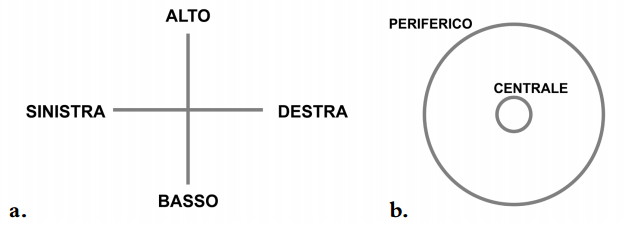
\includegraphics[scale=0.6]{img/012.png}
			\end{center}	
			\caption{Esempi di categorie topologiche: a. alto/basso, sinistra/destra, b. centrale/periferico}
		\end{figure}
\end{itemize}
Quando una figura plastica, o un loro insieme, è tale da assumere un significato all'interno della composizione , allora si parla di formanti plastici. Il formante plastico può rimandare a un significato attraverso due tipi di correlazione tra segno e contenuto:
\begin{itemize}
	\item \textbf{Correlazione simbolica}: si verifica quando esiste una correlazione diretta tra un'unità dell'espressione e un'unità del contenuto, ad esempio:
		\begin{center}
			oro = sacro \\
			("oro" sta a sacro)
		\end{center}
		In questo caso al colore "oro" è associato il significato diretto di "sacro", pertanto all'interno dell'immagine varrà sempre la relazione segno-significato equivalente a oro-sacro
	\item \textbf{Correlazione semi-simbolica}: si verifica quando esiste una correlazione tra una categoria dell'espressione e una categoria dell'contenuto, ad esempio:
		\begin{center}
			alto : basso = sacro : profano\\
			("alto" sta a "basso" come "sacro" sta a "profano")
		\end{center}
	In questo caso alla categoria topologica alto/basso corrisponde spazio del sacro/spazio del profano, pertanto all'interno dell'immagine il significato degli elementi varia in base alla loro posizione relativa nella composizione
\end{itemize}

\subsection{Segni: simboli, icone, pittogrammi}
Una volta definito il segno e capita la sua struttura, possiamo riconoscere diversi tipi di segno, ciascuno differente dall'altro in base alla relazione tra i due componenti, ovvero \textit{significante} e \textit{significato}. \\
Peirce suddivide i segni in tre tipologie:
\begin{itemize}
	\item \textbf{icona}: quando il significante ha un rapporto di analogia con il significato che rappresenta e lo imita. Ne sono un esempio i pittogrammi, le fotografie, e così via.
	\item \textbf{indice}: quando il significante ha un rapporto di causa/effetto con il significato. Il concetto "fuoco" può avere per esempio due indici: il fumo (visivo) e il crepitio delle fiamme (sonoro).
	\item \textbf{simboli}: quando il significante ha un rapporto convenzionale con il significato. Ne sono un esempio molti cartelli stradali, dove i concetti sono espressi attraverso la rappresentazione di simboli geometrici astratti.
\end{itemize}
Queste tre tipologie vengono declinate anche nel campo della progettazione grafica in altrettante tipologie di segni grafici
\begin{itemize}
	\item \textbf{pittogramma}: come l'icona, quando il significante è una rappresentazione del significato
	\item \textbf{ideogramma}:  come l'indice, quando il significante ha una relazione causa/effetto con il significato
	\item \textbf{logogramma}: quando il significante è un segno costituito da lettere
\end{itemize}

\subsection{Rappresentazione grafica di un'idea}
Il linguaggio scritto fa
ampio uso di parole, che richiedono di essere lette e, spesso, di costruire un nesso logico tra parte anche distanti tra di loro all'interno di un testo. Inoltre le parole sono visivamente simili tra di loro, caratteristica che penalizza il lettore frettoloso o distratto: parole come sì e no hanno un contorno simile e occupano aree equivalenti, malgrado il loro significato sia l'uno l'opposto dell'altro.
Al contrario, gli studi sulla segnaletica stradale hanno confermato che i segni figurativi, ovvero le icone, possono essere riconosciuti nella metà del tempo rispetto a segni composti da scritte. \\
Per costruire il messaggio, in questo caso figurativo, non esiste un manuale, ma è comunque necessario stabilire un processo di trasformazione dell'idea in segno.\\
Horton identifica tre azioni principali che l'utente deve svolgere alla vista di un'icona:
\begin{itemize}
	\item \textbf{Decodificare}:  è il processo tramite cui l'utente apprende il significato di un'immagine
	\item \textbf{Riconoscere}: una volta appreso il significato, è necessario che l'utente riconosca l'immagine e che ne richiami il significato
	\item \textbf{Ricercare}: infine può essere necessario ricercare un'icona in particolare in mezzo a tante altre; questo processo è influenzato sia da quanto l'utente ha ben chiara nella memoria la forma dell'obbiettivo, e quanto l'obiettivo è visivamente distinto dagli altri elementi dell'ambiente circostante
\end{itemize}
Quindi, alcuni principi di cui tenere da conto sono che l'icona sia ben riconoscibile anche quando di dimensioni ridotte (ovvero da pochi millimetri a 2-3 centimetri), deve pertanto permettere all'utente di distinguerne le forme; inoltre le icone devono essere ben distinguibili dall'ambiente, e devono pertanto essere caratterizzate da colori ad alto contrasto reciproco, così che sia possibile riconoscerne più facilmente anche i dettagli. 
Horton suggerisce anche le qualità e le caratteristiche che un'icona dovrebbe avere per essere più efficace ed efficiente:
\begin{itemize}
	\item \textbf{Comprensibile}: innanzitutto l'osservatore deve comprenderne il significato. È la qualità senza dubbio più generica ma determinante.
	\item \textbf{Chiara}:  l'immagine deve essere autoesplicativa, senza richiedere l'accesso a informazioni esterne, e soprattutto limitare il più possibili i fraintendimenti e la confusione.
	\item \textbf{Istruttiva}: l'icona deve guidare l'utente nelle proprie azioni, deve trasmettere un senso di sicurezza e dare tutte le informazioni indispensabili e sufficienti per l'interazione.
	\item \textbf{Distinta}: è indispensabile che ciascuna immagine sia ben distinguibile da altre simili, e che siano messe bene in risalto le differenze che la contraddistinguono, così che non si confonda.
	\item \textbf{Indimenticabile}: l'immagine deve essere memorizzata facilmente; per questo motivo aiuta l'uso di immagini concrete piuttosto che astratte, aggiungendo enfasi ed esagerazione su certi aspetti, introducendo cenni di inusualità e bizzarria, o particolarmente all'attività e all'interazione
in corso.
	\item \textbf{Coerente}: tutti gli elementi all'interno dell'immagine e al suo esterno devono collaborare per comunicare un concetto, aiutando a creare un contesto che aiuti l'utente nell'apprendimento e nell'interpretazione.
	\item \textbf{Familiare}: per ridurre lo sforzo dell'utente nell'apprendimento è consigliato utilizzare immagini quanto più a lui familiari, evitando di ricorrere a immagini esotiche o eccessivamente astratte. L'attinenza più fedele all'ambiente dell'interazione e agli standard più diffusi
aiutano l'utente a prevedere con maggior precisione e sicurezza gli effetti o le funzioni di determinate icone
	\item \textbf{Leggibile}: l'utente deve essere in grado di riconoscere ogni elemento che costituisce l'icona, sia esso testualo o figurativo.
	\item \textbf{Limitata}: è consigliabile limitare il numero di elementi grafici e di restringere il più possibile il contesto in cui l'immagine viene utilizzata, così da rendere più immediato l'apprendimento e il riconoscimento.
	\item \textbf{Compatta}: quasi mai l'icona è l'unico elemento di un'interfaccia, pertanto conviene ridurne il più possibile l'ingombro, così da lasciare spazio anche ad altri elementi (sia figurativi che scritte) e permettere all'utente l'accesso a tutte le informazioni indispensabili e sufficienti.
	\item \textbf{Estendibile}: spesso un singolo elemento può ricoprire molteplici ruoli, pertanto bisogna sempre mantenerlo riconoscibile anche in contesti differenti, nonché con dimensioni diverse.
\end{itemize}
\end{document}